% Source for the figure of the front and the rear coding (sec. 15.6): a
% sorted dictionary of eight strings, its front coding (l_i and the rest),
% its rear coding (r_i and the same rest), and the front coding with
% buckets of b = 4, whose anchors (shaded) are stored whole. Build: make
% figures (in ../build).
\documentclass[border=4pt]{standalone}
\usepackage[T1]{fontenc}
\usepackage{newpxtext,newpxmath}
\usepackage[varqu,varl,scaled=0.95]{zi4}
\usepackage{tikz}
% tikz-ads.tex: the TikZ styles shared by the figures of the memory of the
% manual, \input by each standalone figure: a cell of a vector (cell), the
% cell that an operation touches (touched), a free cell (free), a node of a
% linked structure (node), the labels of indices (index) and of variables
% (var), a pointer (ptr), and \cells and \indices to draw a row of cells.
\usetikzlibrary{arrows.meta,positioning,calc,fit,shapes.multipart}
\definecolor{adsTouched}{RGB}{214,196,236}
\definecolor{adsFree}{RGB}{236,236,236}
\tikzset{
  ads/.style={>={Stealth[length=2mm]},font=\small,
              every node/.append style={inner sep=0pt}},
  cell/.style={draw,minimum width=7mm,minimum height=7mm,
               font=\small\ttfamily,outer sep=0pt},
  touched/.style={cell,fill=adsTouched},
  free/.style={cell,fill=adsFree,text=black!45},
  node/.style={draw,rounded corners=1pt,minimum width=8mm,
               minimum height=6mm,font=\small\ttfamily},
  index/.style={font=\scriptsize\ttfamily,text=black!60},
  var/.style={font=\small\itshape},
  ptr/.style={->,thick}
}
% \cells{name}{x,y}{list}: a row of cells, the first at (x,y), named
% name-0, name-1, ...; each item is text/style, the style one of cell,
% touched and free (e.g., {a/cell,e/touched,/free})
\newcommand{\cells}[3]{%
  \foreach \v/\s [count=\i from 0] in {#3}
    \node[\s] (#1-\i) at ($(#2)+(\i*7mm,0)$) {\v};}
% \indices{name}{n}: the indices 0 .. n-1 under the cells of name
\newcommand{\indices}[2]{%
  \foreach \i in {0,...,\numexpr#2-1\relax}
    \node[index,below=1.2mm of #1-\i] {\i};}

\tikzset{
  wc/.style={cell,minimum width=22mm,anchor=west},
  wt/.style={touched,minimum width=22mm,anchor=west},
  st/.style={font=\small\ttfamily,anchor=west}
}
\begin{document}
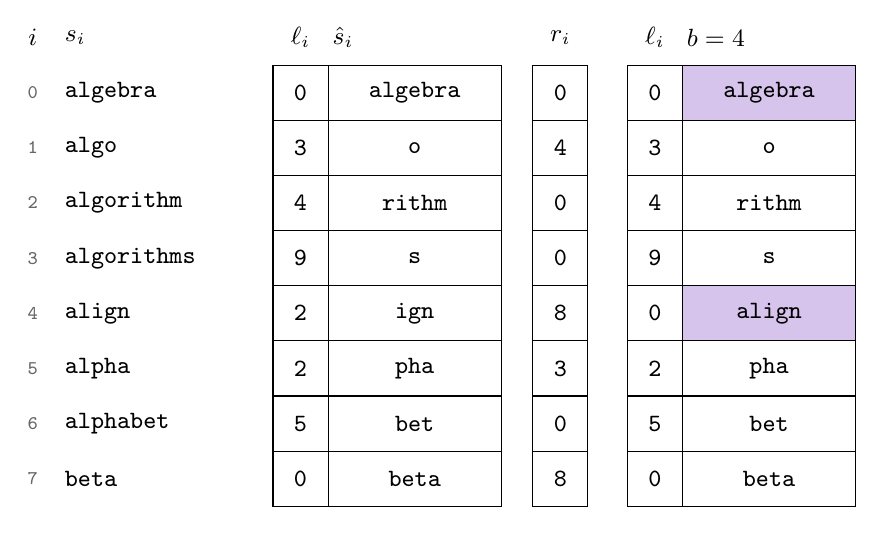
\begin{tikzpicture}[ads]
  \node[var] at (0,7mm) {$i$};
  \node[var,anchor=west] at (4mm,7mm) {$s_i$};
  \node[var] at (34mm,7mm) {$\ell_i$};
  \node[var,anchor=west] at (38mm,7mm) {$\hat s_i$};
  \node[var] at (67mm,7mm) {$r_i$};
  \node[var] at (79mm,7mm) {$\ell_i$};
  \node[var,anchor=west] at (83mm,7mm) {$b = 4$};
  \foreach \i/\s/\l/\r/\rr/\bl/\bs/\st in {
      0/algebra/0/algebra/0/0/algebra/wt,1/algo/3/o/4/3/o/wc,
      2/algorithm/4/rithm/0/4/rithm/wc,3/algorithms/9/s/0/9/s/wc,
      4/align/2/ign/8/0/align/wt,5/alpha/2/pha/3/2/pha/wc,
      6/alphabet/5/bet/0/5/bet/wc,7/beta/0/beta/8/0/beta/wc} {
    \node[index] at (0,-\i*7mm) {\i};
    \node[st] at (4mm,-\i*7mm) {\s};
    \node[cell] at (34mm,-\i*7mm) {\l};
    \node[wc] at (37.5mm,-\i*7mm) {\r};
    \node[cell] at (67mm,-\i*7mm) {\rr};
    \node[cell] at (79mm,-\i*7mm) {\bl};
    \node[\st] at (82.5mm,-\i*7mm) {\bs};
  }
\end{tikzpicture}
\end{document}
